\documentclass{beamer}

% Setup appearance:

\usetheme{Darmstadt}
\usecolortheme{albatross}
\usefonttheme[onlylarge]{structurebold}
\setbeamerfont*{frametitle}{size=\normalsize,series=\bfseries}
\setbeamertemplate{navigation symbols}{}

% Redefine the colors to make them closer to mmm.
\definecolor{MWBlood}{rgb}{0.278, 0.0, 0.016} % MWBlood (primary)
\definecolor{MWBloodDark}{rgb}{0.039, 0.0, 0.0} % MWBloodDark (secondary)
\definecolor{MWBloodMiddle}{rgb}{0.171, 0.00, 0.01} % MWBloodMiddle ()
\definecolor{MWBone}{rgb}{0.827, 0.827, 0.827} % MWBone (Text)

\setbeamercolor*{normal text}{fg=MWBone!50!white,bg=MWBloodMiddle!50!MWBlood} % TOC subsection and more important the dropshadow.
\setbeamercolor*{structure}{fg=MWBlood!25!MWBone} % Section heading color in TOC and inside of enum circles.

\setbeamercolor{palette primary}{bg=MWBlood,fg=MWBone} % Slide heading and title box background.
\setbeamercolor{palette secondary}{bg=MWBloodMiddle, fg=MWBone}
\setbeamercolor{palette tertiary}{bg=green,fg=MWBone}
\setbeamercolor{palette quaternary}{bg=MWBloodDark, fg=MWBone} % Navigation bar
\setbeamercolor{background canvas}{bg=MWBloodDark, fg=green} % Slide background

% Standard packages

\usepackage[T1]{fontenc}
\usepackage[utf8]{inputenc}
\usepackage[greek,english]{babel}
\usepackage{times}
\usepackage{url}
\usepackage{lettrine}
\usepackage{hyperref}

% Setup TikZ

\usepackage{tikz}
\usetikzlibrary{arrows}
\tikzstyle{block}=[draw opacity=0.7,line width=1.4cm]


% Author, Title, etc.

\title[Titel]
{
  \texttt{\huge{meta metal mapper}}\\\vspace{3 mm}
  \textit{A data science and Python journey for software developers}
}

\author[Martin Woelke]
{
  Martin~Woelke
}

\date{Lübeck - \today}

% The main document

\begin{document}

\begin{frame}
  \titlepage
\end{frame}


\section{Introduction}

%\pgfimage[width=.45\textwidth,page=2]{beamer}

  \subsection{Overview}

    \begin{frame}{Summary}
      \tableofcontents
    \end{frame}

  \subsection{meta metal mapper}

    \begin{frame}{What does the quirky name mean?}
      \begin{itemize}
        \item<1->\textbf{Meta} (from the Greek meta- \foreignlanguage{greek}{μετά}- meaning
        "after" or "beyond") is a prefix meaning more comprehensive or transcending.
        \item<2->\textbf{Metal}: A style of contemporary rock  music.
        \item<3->\textbf{Mapper}: An entity making a symbolic depiction emphasizing relationships
        between elements of some space, such as objects, regions, or themes.
      \end{itemize}
    \end{frame}

    \begin{frame}{Origins of metal}
      \begin{center}
        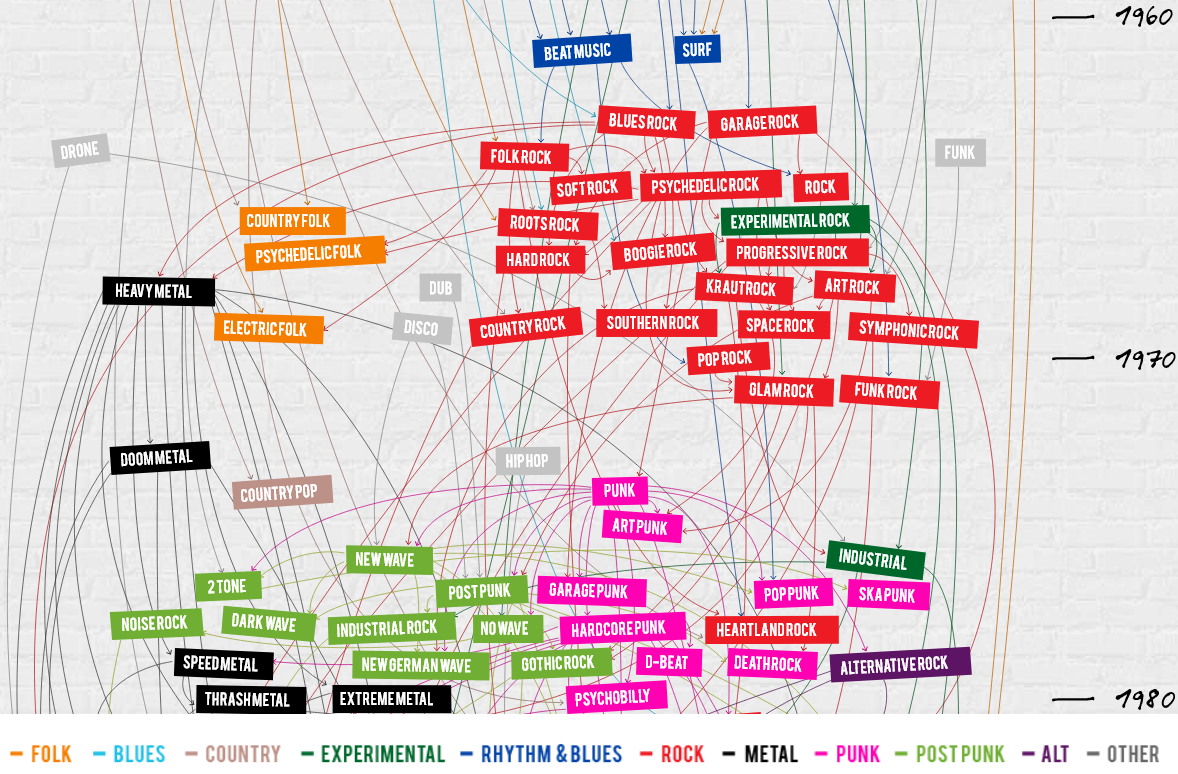
\includegraphics[scale=.33]{familyTree2}
      \end{center}
      \href{https://www.concerthotels.com/100-years-of-rock/}{https://www.concerthotels.com/100-years-of-rock/}
    \end{frame}

    \begin{frame}{What is metal?}
%      \uncover<1-1>
      \pause
      \begin{center}
        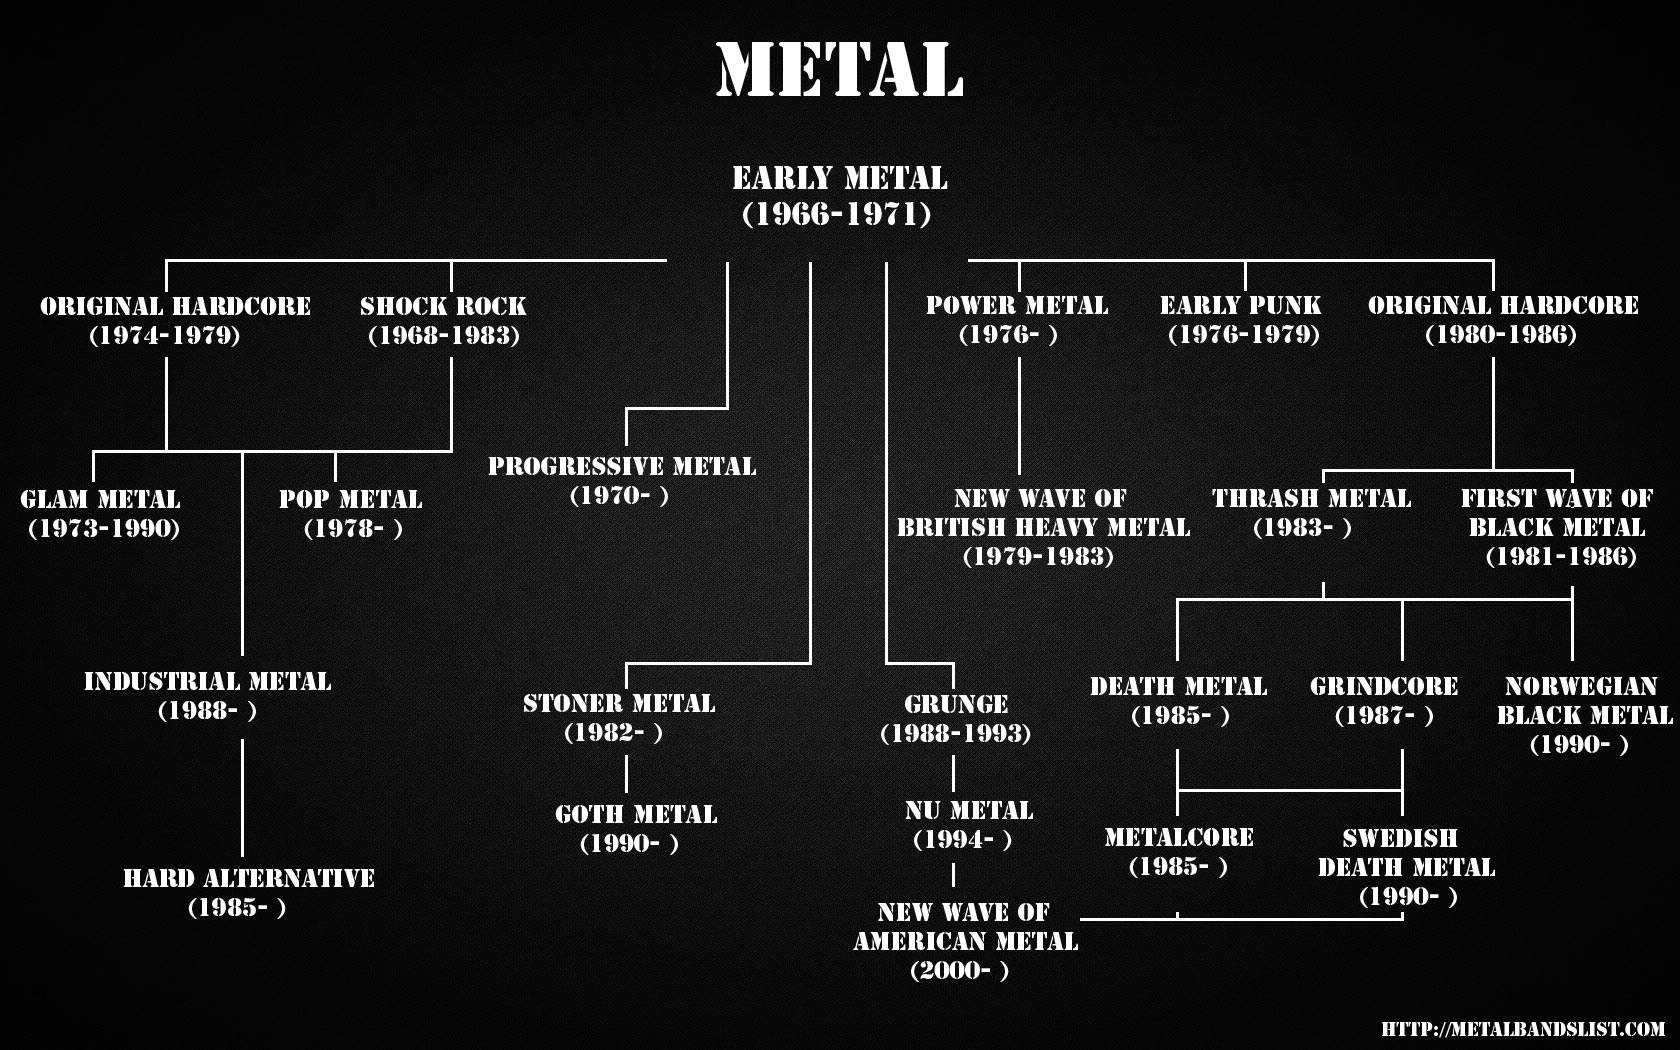
\includegraphics[scale=.18]{familyTree}
      \end{center}
    \end{frame}

    \begin{frame}{What is metal?}

      \begin{block}{Wikipedia Definition}
        Heavy metal (or simply metal) is a genre of rock music that developed in the late 1960s
        and early 1970s, largely in the United Kingdom. With roots in blues rock, psychedelic rock,
        and acid rock, the bands that created heavy metal developed a thick, massive sound,
        characterized by highly amplified distortion, extended guitar solos, emphatic beats,
        and overall loudness.\footnote{https://en.wikipedia.org/wiki/Heavy\_metal\_music}
      \end{block}

    \end{frame}

    \begin{frame}{Inspiration}
      \begin{center}
        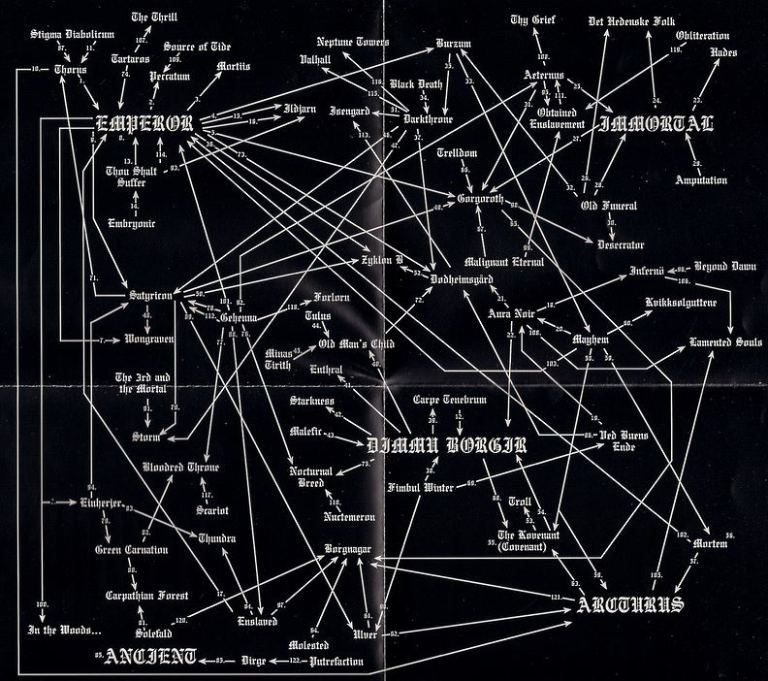
\includegraphics[scale=2.3]{true_kings_diagram}
      \end{center}
    \end{frame}

\section{Development}

    \begin{frame}{History}

      \begin{itemize}

        \item<1-> First commit : 2014-03-15
        \item<1-> Some progress made till July.
          \begin{center}
            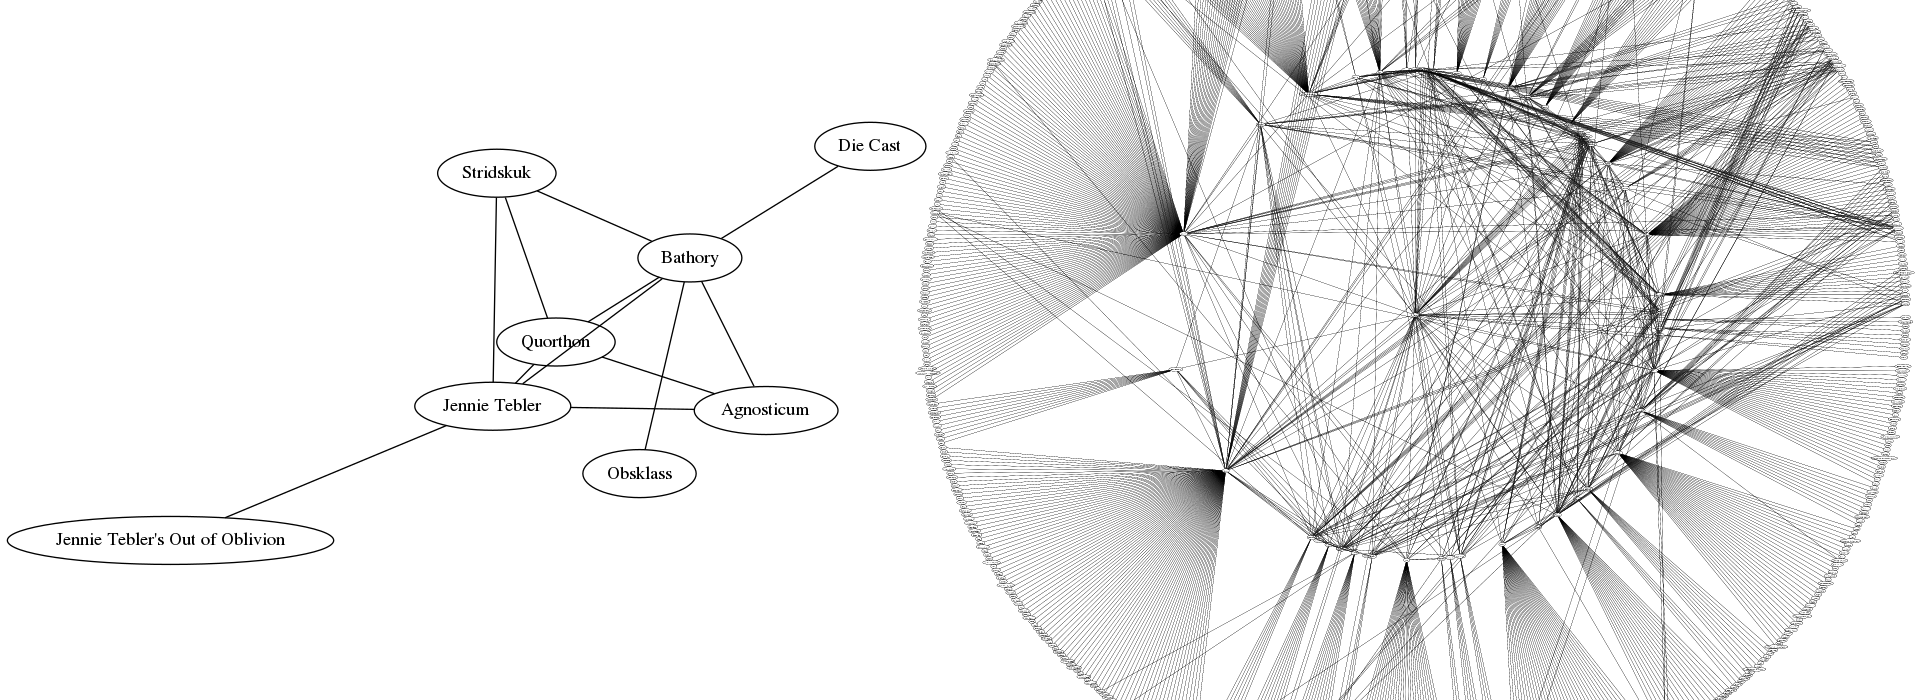
\includegraphics[scale=.6]{bandsGraphCombined}
          \end{center}
        \item<2-> Mothballed until end of 2018.
        \item<2-> 600 Commits later: ~2400 loc + 400 comments + 4k words in
          markdown.
      \end{itemize}

    \end{frame}


%%%%%%%%%%%%%%%%%%%%%%%%%%%%%%%%%%%%%%%%%%%%%%%%%%%%%%%%%%%%%%%%%%%%%%%%%
%%%%%%%%%%%%%%%%%%%%%%%%%%%%%%%%%%%%%%%%%%%%%%%%%%%%%%%%%%%%%%%%%%%%%%%%%

\section{Reporting}

  \subsection{Country Statistics}

    \begin{frame}{Most Common Styles}
      Table?
    \end{frame}

\section{Résumé}

  \subsection{Statistics}

    \begin{frame}{Tools Used}
      \begin{itemize}
        \item<1-> Programming language: Python 2 and 3 on Window and Linux,
        \item<1-> IDEs: Visual Studio and PyCharm,
        \item<1-> Graphviz
        \item<1-> Markdown
        \item<1-> Neo4j (graph database)
        \item<1-> Graphviz (diagram rendering)
        \item<1-> SCM: git
        \item<1-> Gephi (graph rendering and querying)
        \item<1-> \LaTeX{}
        \item<1-> Markdown
      \end{itemize}
    \end{frame}

  \subsection{Link Collection}

    \begin{frame}{Further Reading}
      \begin{itemize}
        \item\href{https://musicmap.info/}{musicmap.info}: Musical genre development (not only metal) and influences over time.
        \item\href{https://www.boundbymetal.com/en/common/metal-genres-graph}: Metal development from the beginning until 2010.
      \end{itemize}
    \end{frame}



\end{document}

    \begin{frame}{}

    \end{frame}


